\documentclass[11pt,english]{article}
\usepackage{authblk}
\usepackage{babel}
\usepackage{hyperref}
\usepackage{cleveref}
\usepackage{graphicx}
\usepackage{algorithm}
\usepackage{algpseudocode}
\date{Monday, April 21st, 2014}
\title{CMPSC440 Final Project Progress Report}
\author[1]{Hawk Weisman}
\author[1]{Dibyojyoti Mukherjee}
\author[1]{Andreas Bach Landgrebe}
\author[2]{Soukaina Hamimoune}
\affil[1]{Allegheny College, Department of Computer Science}
\affil[2]{Al Akhawayn University, Department of Computer Science}
\begin{document}
	\maketitle
	\section{Team Status}
	The Remote Collab team has spent the last week engaged primarily in research, architecture, and design activities in preparation for the implementation of the system.

	Andreas and Soukaina have spent a majority of this time improving their familiarity with the Python programming language, primarily through the use of online tutorials and other resources. Dibyo has been conducting research into the the operational transformation and differential synchronization algorithmic techniques and developing elements of the project architecture, while Hawk has completed setting up the team's continouous integration server and unit testing environment, and has begun implementing the SublimeText plugin.
	\section{Project Status}
	The team has chosen to implement \textit{differential synchronization}, or `diff-sync', using the \textit{dual-shadow method}, as depicted in \Cref{fig:diffsync} and \Cref{alg:diffsync}.
	\begin{figure}
		\centering
		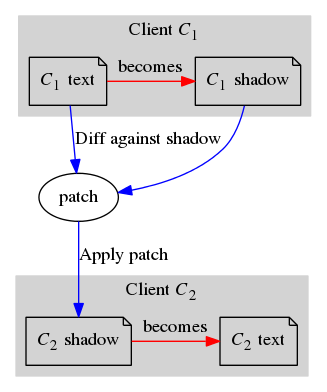
\includegraphics[width=0.5\linewidth]{diffsync.png}
		\caption{Dual-shadow differential synchronization}
		\label{fig:diffsync}
	\end{figure}
	\begin{algorithm}
	\caption{Differential synchronization algorithm}\label{alg:diffsync}
	\begin{algorithmic}[1]
	\Procedure{onViewModified}{$currentBuffer$}
   	\State $currDiff \gets diff(currentBuffer, currentBufferShadow)$
   	\State send($currDiff, pair$)
   	\State $currentBufferShadow \gets currentBuffer$
	\EndProcedure
 	\Procedure{onPatchReceive}{$patch$}
    	\State applyPatch($patch, currentBufferShadow$)
    	\State $currentBuffer \gets currentBufferShadow$
    \EndProcedure
	\end{algorithmic}
	\end{algorithm}
\end{document}